\section{HARDWARE AND SOFTWARE SYSTEM}
\subsection{Structure of Link Module}
We constructed the link module of the multilinks as shown in \figref{hardware}(a). Each link module has a build-in propeller at the center. A servo motor at the end of the link module comprised the main part of the joint module. The rotation range of each joint is $-\frac{\pi}{2}$[rad] $\sim \frac{\pi}{2}$[rad]. The multilinks can transform only in two-dimensions due to the joints with the same rotational axis. The range of lifting force is (0[N]$\sim$16.5[N]). The length of each link is 0.6[m] while the diameter of the propeller protector is 0.38[m]. 
 \begin{figure}[t]
  \begin{center}
    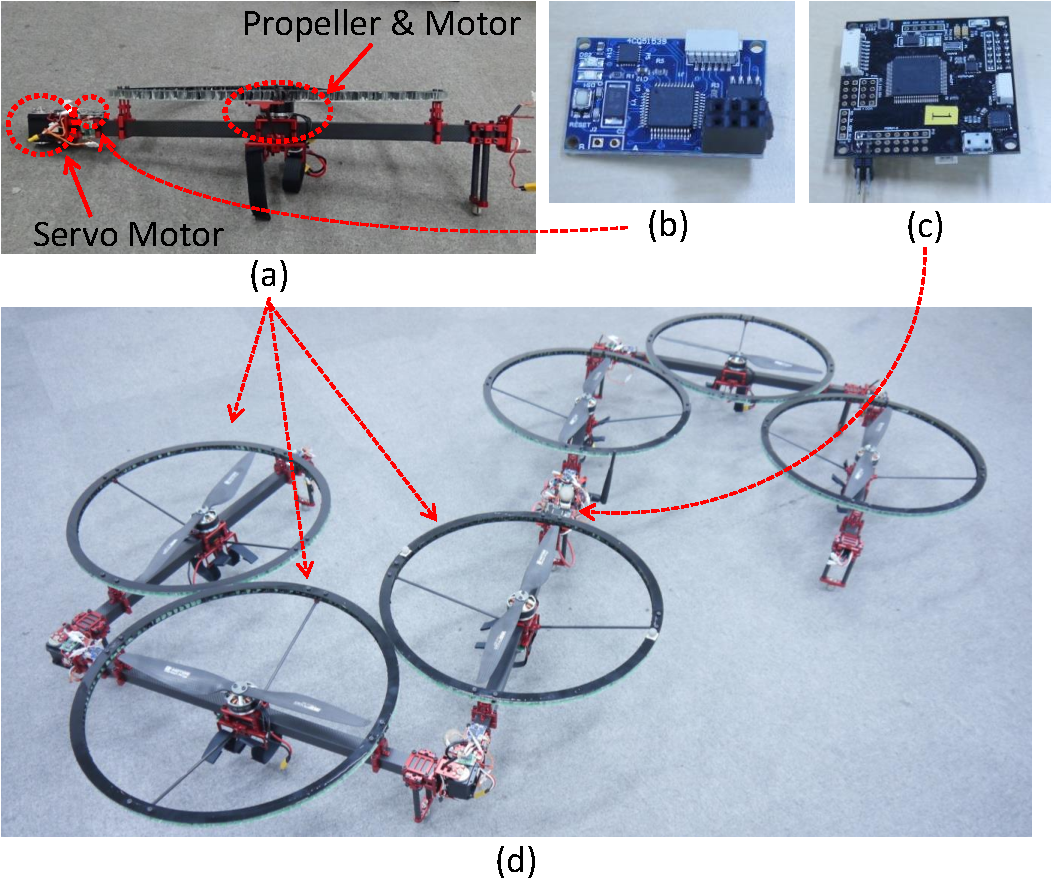
\includegraphics[width=1.0\columnwidth]{figs/hardware.pdf}
  \end{center}
  \caption{The hardware components of the transformable aerial robot. (a): the link module of multilinks with built-in propeller at the center, servo motor at the end and controller board(Neuron). (b): the electromagnet gripper with five electromagnets and four micro switches. (c): transformable hex-rotor with 6-links consisting of the link modules and the electromagnet grippers. \label{figure:hardware}}
\end{figure}

\subsection{Structure of Electromagnet Gripper}
In this work, limiting objects transported by the aerial robot to ferrous objects, we construct an electromagnet gripper(\figref{hardware}(b)). The gripper comprises five electromagnets whose diameter is 20[mm] and four micro switches. Contact with an object can be detected by the signal of micro switches. The electromagnets are driven only while any switch is turned on to save the energy of batteries and to avoid the overheating of electromagnets. As shown in \figref{hardware}(c), the grippers are connected to the aerial robot with strings because the gripper can move passively at the time of contact to an object. The gripper communicates with a computer by using USB-Serial.

\subsection{Multi-Layer Structure for Internal Communication}
The multirotor with multilinks has not only motors for rotation of propeller but also servo motors for transform as actuator. Besides, the length of the multilinks is longer than conventional aerial robots. In the conventional method, an aerial robot has only one central processor connected to all actuators and sensors. However, it is assumed that if we provide the conventional method for the multilinks, the possibility of disconnection increases due to the length of the multilinks. Matsui et al.\cite{Matsui2005} made reference to this problem for humanoid robots.
\par
For the reason noted above, we constructed multi-layer structure for internal communication(\figref{internal_communication}). As shown in \figref{hardware}(a), each link module has the controller board(Neuron)(\figref{controller_board}(a)) which sends data to the motor and the servo motor and receives data from IMU(Inertia Measurement Unit). Moreover, the center link has the other controller board(Spinal)(\figref{controller_board}(b)) which communicates with each Neuron. We use CAN(Controller Area Network)\cite{CAN} to construct the communication system between the controller boards. As used in cars, CAN is a reliable communication system which resists external noise. Thereby, the amount of electric wiring decreases resulting that the reliability of the communication improves. 
\par
Moreover, the computer is connected to Spinal on USB-serial communication. The LQI control, motion planning, etc are executed on the computer.
\begin{figure}[t]
  \begin{center}
    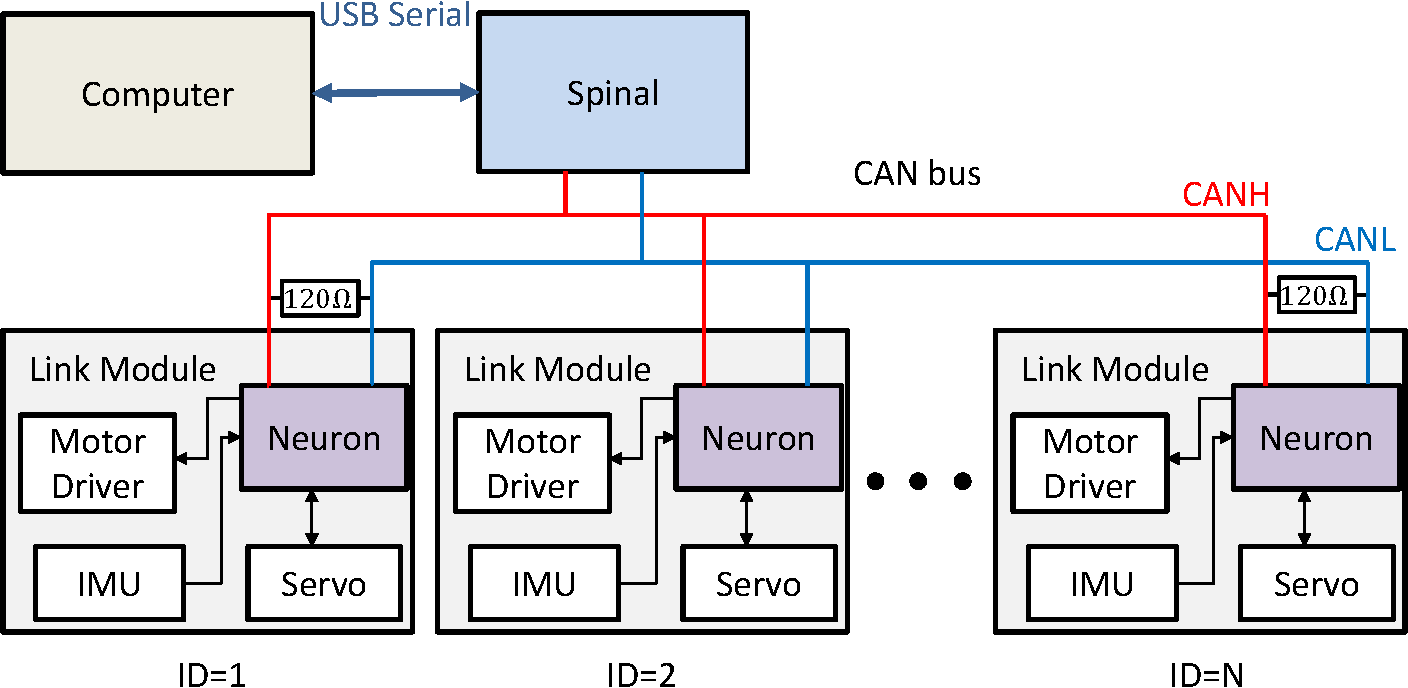
\includegraphics[width=1.0\columnwidth]{figs/internal_communication.pdf}
  \end{center}
  \caption{The multi-layer structure for internal communication comprising Neuron, Spinal and Computer: Neuron communicates with each device(motor, servo motor and IMU) while Spinal communicates with Neuron by using CAN. Computer and Spinal communicate by using USB-Serial.\label{figure:internal_communication}}
\end{figure}
\begin{figure}[t]
  \begin{center}
    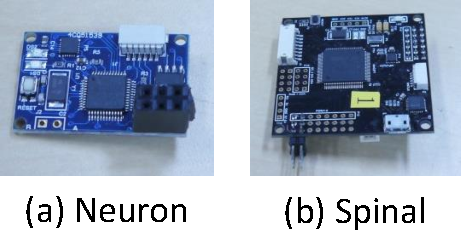
\includegraphics[width=0.7\columnwidth]{figs/controller_board.pdf}
  \end{center}
  \caption{(a): Controller board Neuron communicating with each device and comprising IMU on board. (b): Controller board Spinal communication with each Neuron and the computer.\label{figure:controller_board}}
\end{figure}
